\documentclass{article}


% Use the postscript times font!

% --- Packages ---
\usepackage{times}
\usepackage{ijcai/ijcai17}
\usepackage{enumerate, amsmath, hyperref, amsthm,gensymb, subfig, verbatim, amssymb, dashrule, tikz, bbm, booktabs, bm}
\usepackage[framemethod=TikZ]{mdframed}
\usepackage[numbers]{natbib}

\newcommand{\dnote}[1]{\textcolor{blue}{Dave: #1}}
\newcommand{\enote}[1]{\textcolor{purple}{Emily: #1}}
\newcommand{\mc}{\mathcal}
\newcommand\ddfrac[2]{\frac{\displaystyle #1}{\displaystyle #2}}



% --- Misc. ---
\hbadness=10000 % No "underfull hbox" messages.

% --- Meta Info ---
\title{Improving Solar Panels with Reinforcement Learning}

% Authors
\author{
Emily Reif \\
Department of Computer Science\\
Brown University\\
Providence, RI 02912 \\
\texttt{emily\_reif@brown.edu} \\
\And
David Abel \\
Department of Computer Science\\
Brown University \\
Providence, RI 02912 \\
\texttt{david\_abel@brown.edu} \\
}


% --- Begin Document ---
\begin{document}
\maketitle

% -----------------
% -- Abstract --
% -----------------
\begin{abstract}
Solar panels sustainably harvest energy from the sun. To improve performance, panels are often equipped with a tracking mechanism that computes the sun's position in the sky throughout the day. Based on the tracker's estimate of the sun's location, a controller orients the panel to minimize the angle of incidence between solar radiant energy and the photovoltaic cells on the surface of the panel, increasing total energy harvested. Prior work has developed efficient tracking algorithms that accurately compute the sun's location to facilitate solar tracking and control.
%
However, always pointing a panel directly at the sun does not account for diffuse irradiance in the sky, reflected irradiance from the ground and surrounding surfaces, or changing weather conditions (such as cloud coverage), all of which are contributing factors to the total energy harvested by a solar panel.
%
In this work, we validate the hypothesis that the computational learning paradigm of Reinforcement Learning (RL) can increase the total energy harvested by solar panels by dynamically accounting for these other factors. We advocate for the use of RL for solar panel control due to its {\it effectiveness}, {\it negligible cost}, and {\it versatility}. Our contribution is twofold: (1) adapting typical RL algorithms to the task of improving solar panel performance, and (2) a simulation based on typical solar and irradiance models for experimenting with solar panel control.
%
We evaluate the utility of various RL approaches compared to an idealized tracker, an efficient state of the art tracking algorithm, and a fixed panel in our simulated environment. We experiment across different time scales, in different places on Earth, and with dramatically different percepts (sun coordinates, and synthesized images of the sky with and without clouds), consistently demonstrating that simple RL algorithms improve over existing baselines.
\end{abstract}


% ----------------------
% -- Introduction --
% ----------------------
\section{Introduction}
% Solare Panels and Solar Tracking.
Solar energy offer a pollution free and sustainable means of harvesting energy directly from the sun. Considerable effort has been directed toward maximizing the efficiency of end to end solar systems, including the design of photovoltaic cells~\cite{Jervase2001,li2012molecular}, engineering new photovoltaic architectures and materials~\cite{li2005high}, and solar tracking systems~\cite{camacho2012control}. Solar tracking is especially important for maximizing performance of solar panels~\cite{Eke2012,Rizk2008,King2001}. Given the proper sensors and hardware, a tracking algorithm computes the relative location of the sun in the sky throughout the day and a controller orients the panel to point at the sun. The goal is to minimize the angle of incidence between incoming solar radiant energy and the grid of photovoltaic cells, as in~\citet{Eke2012,Benghanem2011,King2001} and~\citet{kalogirou1996design}. Prior work has consistently demonstrated that panels using a tracking system increase the total energy by a substantial amount:~\citet{Eke2012} report that a dual-axis tracker yielded 71 kW/h, compared to a fixed panel's yield of 52 kW/h on the same day. Eke and Senturk also report energy harvesting gains of dual-axis tracking systems over fixed systems varying from 15\% to 40\%, depending on the time of year.~\citet{mousazadeh2009review} report that gains from tracking can vary between 0\% and 100\%, while~\citet{clifford2004design} report a gain of $23\%$ due to tracking in simulation. Clearly, solar tracking and control can dramatically benefit solar photovoltaic systems.

% Diagram with labels
\begin{figure}[t]
\begin{center}
\includegraphics[scale=0.3]{figures/relevant_quantities.png}
\caption{\dnote{3D Diagram of sun, label relevant angles}}
\end{center}
\end{figure}

% Previous algorithms
Developments in solar tracking have led to algorithms that are sufficiently accurate to inform control of panels, building on the early work of~\citet{spencer1971fourier,walraven1978calculating} and~\citet{michalsky1988astronomical}. Recently,~\citet{reda2004solar} developed an algorithm that computes the sun's location in the sky within $\pm 0.0003\degree$ of accuracy, achieving the highest degree of accuracy of any known algorithm, but is computationally inefficient to the point of impracticality.~\citet{Grena2008} overcomes these inefficiencies with a tracking algorithm that requires an order of magnitude fewer calculations than the approach of Reda and Andreas, while achieving $0.0027\degree$ of accuracy.

% Limitations
However, prior literature suggests that a variety of factors contribute to the performance of a panel~\cite{King2001}, and so pointing a panel directly at the sun is not always optimal behavior. Specifically, the total solar irradiance falling on a panel is a combination of {\it direct}, {\it reflective}, and {\it diffuse} irradiance~\cite{Benghanem2011}. The diffuse irradiance typically varies between $15\%$ and $55\%$ of direct irradiance depending on factors like cloud coverage and the time of day~\cite{peterson1981ratio}, while a case study by the Cold Climate Housing Research Center in Fairbanks, Alaska reports reflective irradiance varying from $5\%$ to $25\%$ of direct irradiance~\cite{colgan2010}. The reflective irradiance varies heavily based on the percentage of irradiance reflected off the surrounding ground surface: typical values for this percentage given by~\citet{mcevoy2003practical} vary between $17\%$ (soil), $25\%$ (grass), and $55\%$ (concrete). Additionally, changing weather and atmospheric conditions can affect the optimal panel orientation~\cite{Kelly2009}. Thus, optimal performance may involve prioritizing reflective or diffuse irradiance when direct sunlight is not available.

% Others require extra hardware.
As an additional consideration, tracking algorithms take as input a variety of data that require additional hardware such as a barometer, thermometer, or GPS~\cite{Grena2012}, increasing the total cost and system complexity.\footnote{Some tracking algorithms do not require the temperature and pressure but incur a cost of accuracy, such as Algorithm 1 from~\citet{Grena2012}.}

% RL for solar tracking.
In this work, we advocate for the use of the computational paradigm of Reinforcement Learning (RL) to optimize solar panel performance. Using RL, a learned solar panel controller can account for weather change, cloud coverage, and diverse reflective indices of surroundings, offering an efficient yet adaptive solution that can optimize for the given availability of each type of solar irradiance without the need for complex hardware. Our primary contribution is twofold:
\begin{enumerate}
\item The advancement of a highly relevant problem as an application area for RL, along with a high fidelity simulation for evaluation built using recent models of solar irradiance.
\item The validation of the utility of RL approaches for solar panel control.
\end{enumerate}

% ----------------------
% -- Background --
% ----------------------
\section{Background}

First, some background on solar tracking and RL.

% Solar Tracking Background
\subsection{Solar Tracking}
The amount of solar radiant energy contacting a surface on the Earth's surface (per unit area, per unit time) is called {\it irradiance}~\cite{goswami2000principles}.  We denote the total irradiance hitting a panel as $R_t$, which, per the models developed by~\citet{kamali2006estimating}, is approximated by the sum of the {\it direct} irradiance, $R_d$, {\it diffuse} irradiance (light from the sky), $R_f$, and {\it reflective} irradiance, $R_r$ (reflected off the ground or other surfaces). Each of these components is modified by a scalar, $\theta_d, \theta_f, \theta_r \in [0,1]$, denoting the effect of the angle of incidence between oncoming solar rays and the panel's orientation, yielding the total:
\begin{equation}
R_t = R_d \theta_d + R_f \theta_f + R_r \theta_r
\label{eq:total_rads}
\end{equation}
Additionally, the components $R_d$ and $R_f$ are known to be effected by cloud coverage~\cite{li2004overcast,pfister2003cloud,tzoumanikas2016effect}. We attend to these details in describing our simulation in Section~\ref{sec:simulation}.

% Controller for solar panel.
A controller for a solar panel then seeks to maximize total irradiance, $R_t$, hitting the panel's surface. In the case of solar trackers, a running assumption is that optimal behavior is generally to point the panel such that its normal vector is pointing at the sun, thus the desire for accurate solar tracking algorithms. There are many types of tracking and control methods, only a few of which we discuss in this work; for an in depth survey of solar tracking techniques, see~\citet{mousazadeh2009review}.

% --- Table of Quantities ---
{\renewcommand{\arraystretch}{1.2}%
\begin{figure}
\centering
\begin{tabular}{lcc}
\toprule
Quantity& Variable& Range \\
\midrule
latitude& $L$& $[-\pi, \pi]$ \\
longitude& $G$&  $\left[-\frac{\pi}{2}, \frac{\pi}{2}\right]$\\
declination& $\delta$ & $\left[-\frac{\pi}{2}, \frac{\pi}{2}\right]$ \\
hour angle& $H$& $\left[-\frac{\pi}{2}, \frac{\pi}{2}\right]$ \\
%zenith& $z$& $[0,\pi]$ \\
azimuth& $\Gamma$& $[-\pi, \pi]$ \\
altitude& $\alpha$& $[-\pi, \pi]$ \\
panel NS angle& $\nu$& $[-\pi, \pi]$ \\
panel EW angle& $\omega$& $[-\pi, \pi]$ \\
ground reflective index& $\rho$& $[0,1]$ \\
\bottomrule
\end{tabular}
\caption{Relevant solar tracking and irradiance variables.}
\end{figure}

% RL Background
\subsection{RL Background}

Reinforcement Learning (RL) is a computational learning paradigm in which an agent learns to maximize an unknown reward function through repeated interaction with the agent's environment. In this work we model the environment as a Markov Decision Process (MDP)~\cite{puterman2014markov}. An MDP is a five tuple, $\langle \mc{S}, \mc{A}, \mc{R}, \mc{T}, \gamma \rangle$, where:
\begin{enumerate}
\item $\mc{S}$ is a set of states
\item $\mc{A}$ is a set of actions
\item $\mc{R} : \mc{S} \times \mc{A} \longmapsto [0,\textsc{RMax}] $ is a reward function.
\item $\mc{T}(s' \mid s,a)$ is a probability distribution on states given a state and action
\item $\gamma \in (0,1)$ is a discount factor, indicating how much the agent prefers immediate reward over future reward.
\end{enumerate}

The solution to an MDP is called a {\it policy}, denoted $\pi : \mc{S} \longmapsto \mc{A}$. The goal of an agent is solve for a policy that maximizes long term expected reward, defined by the {\it value function}, $V^* : S \longmapsto \left[0,\frac{\textsc{RMax}}{1-\gamma}\right]$, given by the classic Bellman Equation:
\begin{equation}
V^*(s) = \max_a \left(\mc{R}(s,a) + \gamma \sum_{s'} \mc{T}(s' \mid s, a) V^*(s') \right)
\end{equation}

Also of interest is the {\it action-value function}, $Q^*: \mc{S} \times \mc{A} \longmapsto [0,\textsc{RMax}]$, which specifies the long term expected reward of executing an action in a state, and behaving optimally thereafter:
\begin{equation}
Q^*(s,a) = \mc{R}(s,a) + \gamma \sum_{s'} \mc{T}(s' \mid s,a) V^*(s')
\end{equation}

Given a policy, $\pi$, the value under the policy is defined by:
\begin{equation}
V^\pi(s) = \mc{R}(s, \pi(s)) + \gamma \sum_{s'} \mc{T}(s' \mid s, \pi(s)) V^\pi(s')
\end{equation}

For further background on RL, see~\citet{sutton1998reinforcement} or~\citet{kaelbling1996reinforcement}.

% Agents
\subsubsection{Agents}
We evaluate two relatively simple agents (and variations thereof): $Q$-Learning with a Linear Function approximator with a Gaussian radial basis kernel and $SARSA$ with a linear function approximator. To test the significance of modeling the sequential aspects of the problem, we also conduct experiments with LinUCB~\cite{li2010contextual}, a standard approach to Contextual Bandits. We chosen each of the linear approximators to illustrate that online, efficient, and lightweight algorithms can be effective in the domain.

$Q$-Learning, introduced by~\citet{watkins1992q}, updates the $Q$ function via one step look aheads each experience, $\langle s, a, r, s' \rangle$, according to the gradient update rule:
\begin{equation}
Q(s,a) = (1-\eta) Q(s,a) + \eta(r + \gamma \max_{a'} Q(s', a'))
\end{equation}
Where $\eta \in [0,1]$ is a learning rate. The linear approximation scales tabular $Q$ learning to domains where states or observables are described by a high dimensional feature vector, $s = [s_1, s_2, \ldots, s_k]$. The $Q$ function is parameterized by the matrix $\theta$, where each column corresponds to an action's parameters, and each row is a state variable. and computes the $Q$ value as:
\begin{equation}
Q_\theta(s,a) = \sum_{i=1}^k \theta_{i,a} s_i
\end{equation}
The parameters are updated via the gradient update rule, again given a single experience $\langle s, a, r, s' \rangle$:
\begin{equation}
\theta_{i,a} = \theta_{i,a} + \eta \left( r + \gamma \max_{a'} Q_\theta(s',a') - Q_\theta(s,a)\right)
\end{equation}

To introduce some non-linearity, we apply a Gaussian radial basis kernel to each feature. That is, let:
\begin{equation}
\phi(s_i) = e^{-(s_i^2)}
\end{equation}
The agent receives states passed through this kernel:
\begin{equation}
\phi(s) = [\phi(s_1), \phi(s_2), \ldots, \phi(s_k)]
\end{equation}

We also test with SARSA~\cite{rummery1994line}, again with a Linear Function Approximator. The only difference from the $Q$-Learner is the update rule. The algorithm updates using the chosen next action $a'$, instead of the max:
\begin{equation}
\theta_{i,a} = \theta_{i,a} + \alpha \left( r + \gamma Q_\theta(s',a') - Q_\theta(s,a)\right)
\end{equation}
Due to the online nature of the true panel control problem, SARSA is attractive as an approach on account of its on policy learning.

% Contextual Bandits
\subsubsection{Contextual Bandits}

A simplification of the full RL problem is a non-sequential variant known as the Contextual Bandit introduced by~\citet{wang2005bandit}, which extends of the classic Multi-Armed Bandit problem~\cite{gittins1979bandit}. In the Contextual Bandit setting, the agent receives a {\it context matrix} $\bm{x}$ containing a feature vector for each action. That is, each column of $\bm{x}$ corresponds to each action's context: the entry $\bm{x}_{i,j}$ denotes the $i$-th feature of action $a_j$. At each time step, the agent chooses an action $a \in \mc{A}$, and receives payoff according to an unknown, possibly stochastic function, $R(\bm{x},a)$. Here, agents still face the exploration-exploitation dilemma but do not need to compute complex causal models of their environments or learn from delayed reward.

Here we adopt the bandit framework to solar panel control to test the significance of modeling the problem as sequential. Each context is simply the received percept from the environment (there is no difference in contexts across actions). Due to its simplicity and efficiency, we experiment with the LinUCB algorithm developed by~\citet{li2010contextual}.

LinUCB adapts the core ideas of Upper Confidence Bound (UCB) algorithm~\cite{auer2002finite} to deal with contexts; in particular, LinUCB explicitly tracks the uncertainty associated with each action using a disjoint linear model. This uncertainty is then factored into an overall computation of the {\it score} associated with each action. At each round, the agent then selects the action with maximal score.

\dnote{Details on UCB?}

%LinUCB was originally adopted for cases with linear payoff matrices:
%\begin{equation}
%\mathbb{E}\left[r \mid \bm{x}, a\right] = \bm{x}^\top \bm{\theta}_a
%\end{equation}
%Where $\bm{\theta}_a$ is an unknown coefficient vector. 

We now turn to describing the details of our simulation.

% ----------------------
% --- Simulation ---
% ----------------------
\section{Simulation}
\label{sec:simulation}

We introduce a high fidelity simulated environment to test the validity of RL for solar panel control. There are four basic stages to the simulation:
\begin{enumerate}
\item Computing the sun's location in the sky, relative to the panel.
\item Computing $R_d, R_f$, and $R_r$.
\item Computing $\theta_d, \theta_f$, and $\theta_r$.
\item Generating percepts.
\end{enumerate}

% (Step 1) Sun location in the sky.
\subsection{Sun's location in the sky}
For a given latitude, longitude, year, month, day, and time, we simulate the relative positions of the sun to the specified location on Earth. Our simulation computes the sun's altitude $\alpha$ (angle: degrees above the horizon) and azimuth $\Gamma$ (angle: clockwise degrees along the horizon relative to North) using using the highly accurate tracker algorithm from~\citet{reda2004solar}, implemented in the library \texttt{pysolar}.\footnote{\url{pysolar.org}}. For space constraints, we do not divulge the full computations. Instead, note that a quick approximation is given by:
% --- Math about \alpha and \Gamma ---
\begin{align}
\alpha &= \arcsin(\cos L \cos \delta \cos H + \sin L \sin \delta)\\
\Gamma &= \arcsin\left(\frac{\cos \delta \sin H}{\cos \alpha}\right)
\end{align}
For the full details, see~\citet{reda2004solar}.

% (Step 2) Irradiance.
\subsection{Computing $\pmb{R_d, R_f, R_r}$}
Given the sun's altitude, $\alpha$, and azimuth, $\Gamma$, we compute the $R_d, R_f,$ and $R_d$ from the models of~\citet{threlkeld1957direct,Liu1960} and~\citet{masters2013renewable}.\footnote{Higher fidelity models are known to exist, such as those developed by~\citet{andersen1980comments,klein1977calculation} and~\citet{kamali2006estimating}. In particular, our estimates of the diffuse and reflective radiation are simple relative to the best known models (this choice was made to make the simulation more efficient).}
% --- Math about R_d, R_f, R_r ---
\begin{align}
R_d &= A e^{-km} \\
R_f &= C \cdot R_d \\
R_r &= \rho R_d (\sin \alpha + C)
\end{align}
Where $A$ is the apparent extraterrestrial flux, $k$ is the optical depth, $m$ is the air mass ratio, $\rho \in [0,1)$ is a reflective index (albedo) denoting how reflective the ground is,\footnote{Typical values for $\rho$ given by~\citet{mcevoy2003practical} vary between 0.17 (soil), 0.25 (grass), and 0.55 (concrete).} and $C$ is a sky diffusion factor, each given by the approximations:
\begin{align}
m&=\frac{1}{\sin \alpha} \hspace{4mm} A = 1160 + \sin \left(0.99 n- 271\right)\\
k&=0.174 + 0.035 \sin\left( 0.99 n - 99\right)\\
C&=0.095 + 0.04 \sin\left(0.99 n-99\right)
\end{align}
Where $n \in [1:365]$ is a day of the year.

% (Step 3) angles.
\subsection{Computing $\pmb{\theta_d, \theta_f, \theta_r}$}
Given the angles describing the panel's orientation ($\nu$: north-south tilt, $\omega$: east-west tilt), we then simulate the amount of total irradiance actually hitting the panel's surface, given the panel's orientation relative to the sun. The models of~\citet{masters2013renewable} define this angle of incidence as the $\cos$-similarity between the panel's normal vector and the sun's vector (with the panel as the origin):
% --- Math about \theta_d, \theta_f, \theta_r. ---
\begin{align*}
\vec{p} &= \left[ \sin(\nu)  \cos(\omega), \cos(\nu)  \cos(\omega), \cos(\nu) \cos(\omega) \right] \\
\vec{s} &= \left[ \sin(\pi - \Gamma)  \cos(\alpha), \cos(\pi - \Gamma)  \cos(\alpha), \sin(\alpha) \right]
\end{align*}
We then compute $\theta_d$ as follows:
\begin{multline}
\theta_d = \frac{\vec{p} \cdot \vec{s}}{||\vec{p}|| ||\vec{s} ||} = \sin(\nu)  \cos(\omega)  \sin(\pi - \Gamma)  \cos(\alpha)\ + \\
\cos(\nu)  \cos(\omega)  \cos(\pi - \Gamma)  \cos(\alpha) +  \cos(\nu) \cos(\omega)  \sin(\alpha) 
\end{multline}

The diffuse irradiance incident angle, $\theta_f$, is given by a simple approximation: the solar collector is exposed to whatever fraction of the sky it points to, while $\theta_r$ is given by the fraction of the ground the collector points to:
\begin{equation}
\theta_f = \frac{\cos \nu + \cos \omega}{2}, \hspace{4mm} \theta_r = \frac{2 - \cos\nu - \cos \omega}{2}
\end{equation}

% Sample Percepts
\begin{figure}[t]
\begin{center}
\subfloat[Sample Sky Percepts\label{fig:sun_image}]{
	\includegraphics[scale=0.20]{figures/sun_img} \hspace{2mm}
	\includegraphics[scale=0.20]{figures/sun_img2}
} \hspace{16mm} % Sun image.
\subfloat[Sample Sky + Cloud Percepts\label{fig:sun_image_clouds}]{
	\includegraphics[scale=0.20]{figures/cloud_img} \hspace{2mm}
	\includegraphics[scale=0.20]{figures/cloud_img2}	
} % Clouds.
\caption{Example percepts given to the RL agent with no clouds (top) and simulated cloud coverage (bottom).}
\end{center}
\end{figure}

% (Step 4) Percepts
\subsection{Generating Percepts}

The final step in the simulation is to generate percepts for the RL agents and Bandit algorithm.\footnote{The tracking algorithm always receives the same information: the year, month, day, hour, longitude, and latitude.} Our most immediate plan for future work is to build a physical system to conduct experiments with RL outside of simulation. In the real setting, we plan on equipping each solar panel with a fish eye monocular camera to provide images of the sky as input for the RL algorithm. To approximate the real setting, our simulated environment supports generating percepts of three kinds:
\begin{enumerate}
\item The panel's orientation and two angles representing the sun's true position in the sky, relative to the panel (four state variables).
\item A $16 \times 16$ synthesized grayscale image of the clear sky ($256$ state variables, each in the range $[0,1]$).
\item A $16\times 16$ synthesized grayscale image of the sky with simulated cloud cover ($256$ state variables, each in the range $[0,1]$).
\end{enumerate}
Naturally, the dimensions of the image can be controlled. For both image percepts, the sky angle changes as the panel moves (estimating the behavior of having a fixed camera mounted to the panel).

Cloud cover is created by generating small Gaussian blobs in the synthesized images, which we then use to modify the direct irradiance that reaches the panel's surface, approximating cloudy weather conditions. The cloudy conditions are randomized each morning at 4am, with the clouds moving across the sky throughout the course of the day. Surprisingly, studies demonstrate that diffuse irradiance can be magnified by cloud cover~\cite{robinson1966solar}, but cloud cover can also decrease diffuse irradiance depending on conditions~\cite{pfister2003cloud}. Direct irradiance $(R_d)$, however, is almost always decreased by cloud cover. Thus, if a cloud sits between the panel and the sun, we reduce the direct irradiance hitting the panel's surface by a factor proportional to the clouds intensity but choose not to impact the diffuse irradiance. Each cloud is modeled as a Multivariate gaussian, with $\mu$ and $\Sigma$ randomized on creation of the cloud, and the intensity of the cloud corresponds to the value of the Gaussian. In most experiments involving cloud cover, the clouds reduce the direct irradiance by anywhere from $10\%$ to $90\%$.

% ----------------------
% -- Experiments --
% ----------------------
\section{Experiments}

% \url{https://github.com/david-abel/simple_rl}
We wrap these four steps inside of a Markov Decision Process (MDP) using the open source library \texttt{simple-rl}.\footnote{{\it Link redacted during review.}}. Each action of the MDP, $a \in \mc{A}$ is one of $\{\texttt{tilt N},\ \texttt{tilt E},\ \texttt{tilt S},\ \texttt{tilt W},\ \texttt{nothing}\}$. Executing the \texttt{nothing} action keeps the panel orientation fixed, while the other four each shift the panel $2\degree$ in their respective directions. Each time step is equivalent to three minutes of time passing (which is a tunable parameter). We let $\gamma=0.99$.

Our core algorithms are $Q$-Learning with a Linear Function approximator, tested with (\texttt{ql-linear-rbf}) and without (\texttt{ql-linear)} a Gaussian radial basis function kernel to introduce some non-linearity, and SARSA with a linear function approximator with a Gaussian radial basis kernel (\texttt{sarsa-linear-rbf}). Each of these algorithms uses $\varepsilon$-greedy exploration with $\varepsilon$ set to $0.2$ and learning rate $\eta = 0.1$ with a standard annealing schedule. The LinUCB approach (\texttt{lin-ucb}) uses an uncertainty bound of $0.5$.

Our core benchmark algorithm is Algorithm 2 from~\citet{Grena2012}, an efficient but accurate solar tracking algorithm, coupled with a controller that always points perfectly at the tracker's estimate of the sun's location. We also provide results for a fixed panel to illustrate the importance of tracking (\texttt{fixed}), and a highly idealized tracker that computes the perfect orientation at each time step to illustrate an upper bound on performance (\texttt{optimal}), and to visualize the degree of suboptimality of the other approaches.

\subsection{Primary Experiments}
We conduct three primary experiments, each with different percepts. In all experiments, all algorithms are trained online in that they never see the same state twice, presenting an especially difficult challenge for the RL agents. Each experiment is run in simulation, once in Mildora, Australia, in June 2015, and once in Reykjavik, Iceland during August 2018. The tracker is always given the data needed to estimate the location of the sun, while the percepts change for the RL agent. In the first experiment, the RL agents are given the true sun angles, $\alpha$ and $\Gamma$, and the panel's tilt angles, $\omega$ and $\phi$. The second experiment is intended to more accurately approximate solar tracking in the real world: the RL agents are synthesized greyscale image of the sky taken from the panel's tilted position, shown in Figure~\ref{fig:sun_image}. In the final experiment, the RL agents perceive a bitmap of the sky with simulated cloud coverage shown in Figure~\ref{fig:sun_image_clouds}. The reward function for all three experiments is given by Equation~\ref{eq:total_rads}, where the third experiment incorporates a small effect of cloud coverage on $R_d$. In all experiments we set the reflective index ($\rho$) to $0.5$.

All of our code for running experiments and for reproducing results is publicly available.\footnote{{\it Link redacted during review.}} %\url{https://github.com/david-abel/solar_panels_rl/experiments}}.

\subsection{Supplementary Experiments}
We also conduct two supplementary experiments. The first investigates the learning speed and performance difference between a single vs. double axis controller, and the second compares the effect of different reflective indices on overall performance. For both experiments we evaluate in New York City, NY during the first five days of November 2025. We only run a subset of the algorithms on each of these experiments to best illustrate the effects of the variable of interest (number of axes, magnitude of $\rho$). For the reflective index experiment, we test with $\rho \in \{0.1,0.5,0.9\}$.

% ------------------
% --- Results ---
% ------------------
\subsection{Results}




% Results (Mildura)
\begin{figure*}[t]
\begin{center}
	\subfloat[True Sun Angles]{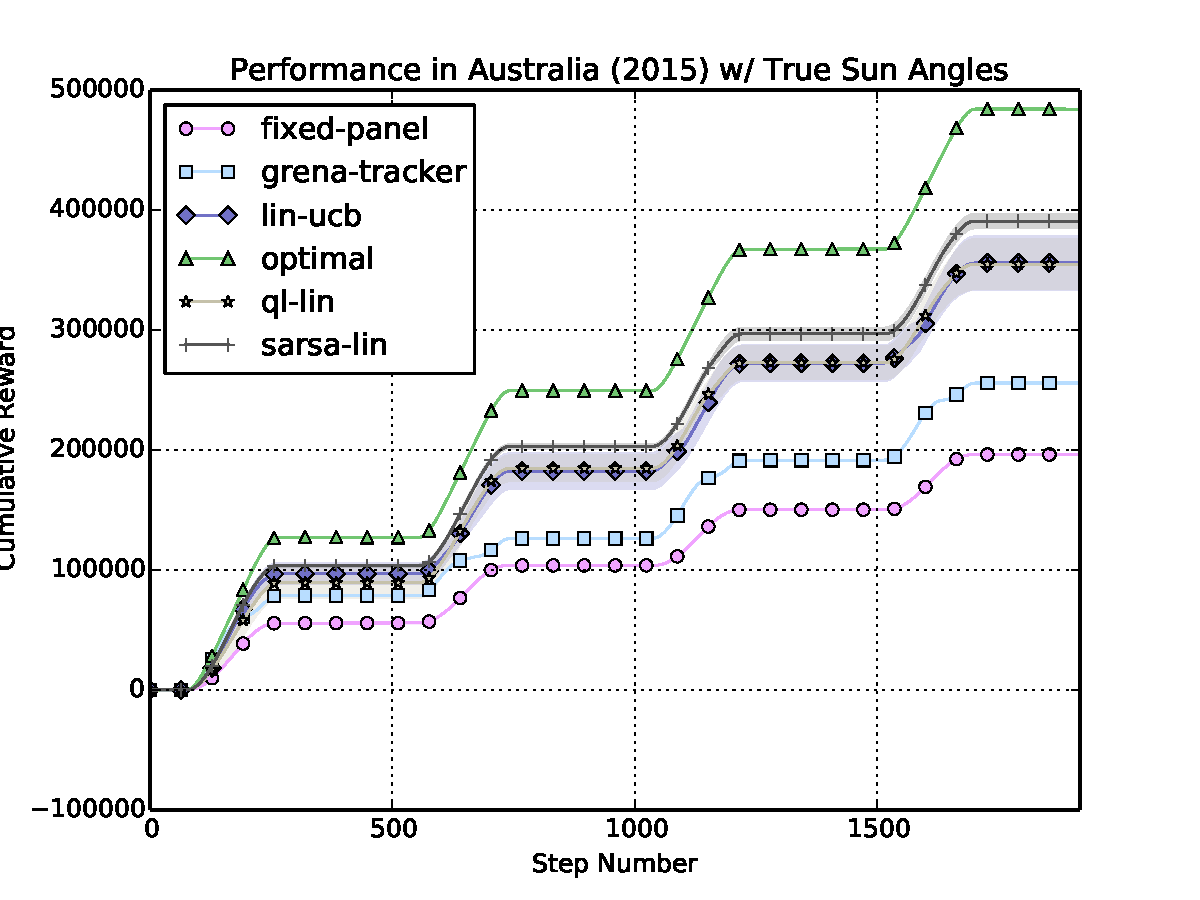
\includegraphics[scale=0.26]{figures/mildura/true_cumulative}} \hspace{1mm}% True sun angles percept.
	\subfloat[Bitmap of the Sky]{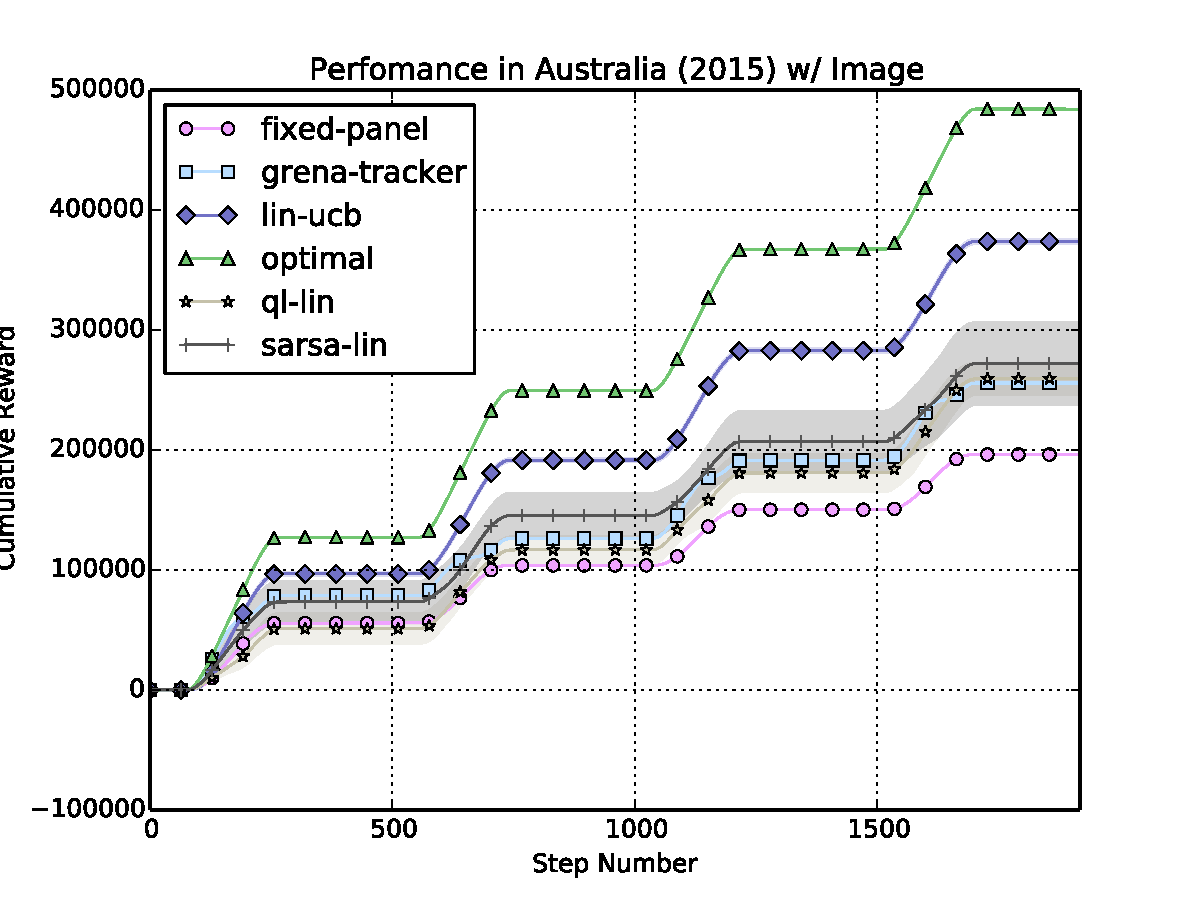
\includegraphics[scale=0.26]{figures/mildura/img_cumulative}} \hspace{1mm} % Sun image percept.
%	\subfloat[Bitmap of the Cloudy Sky]{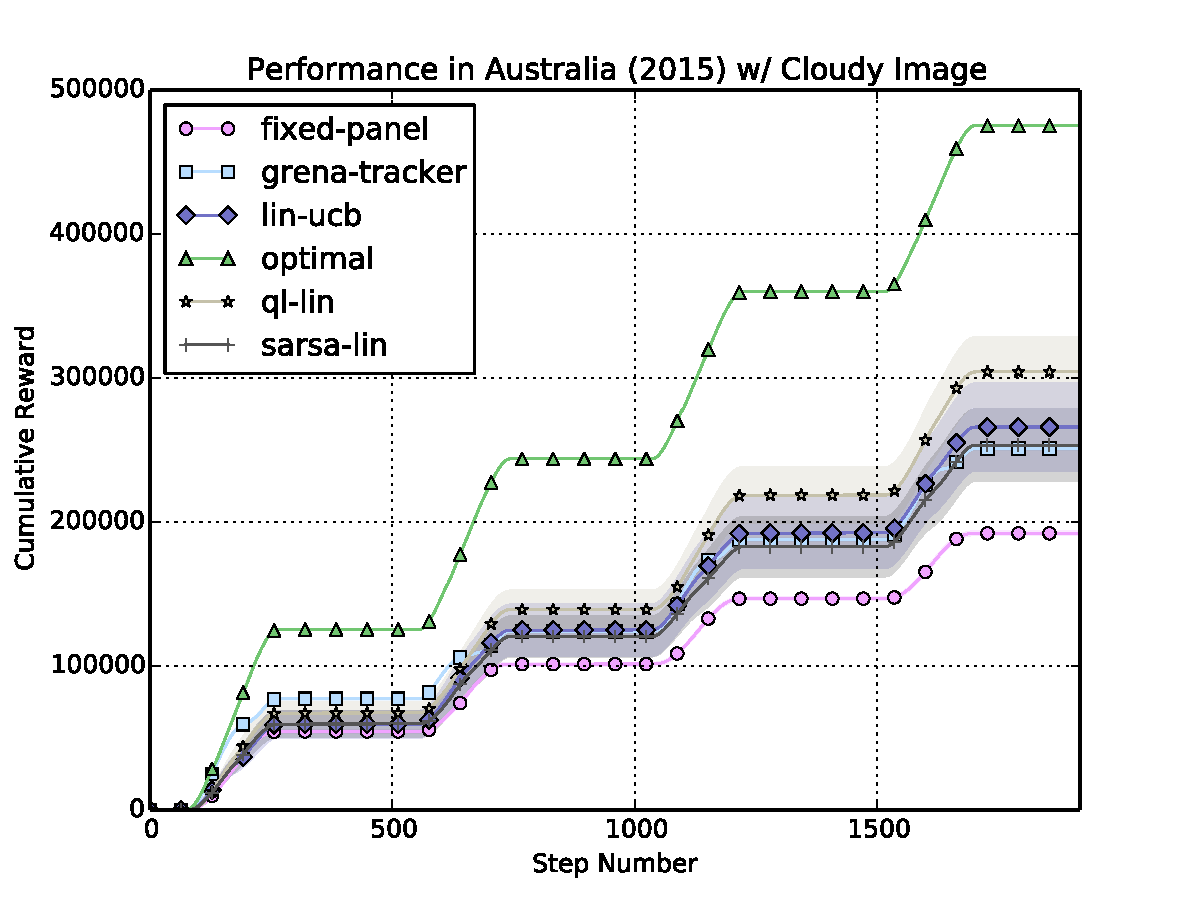
\includegraphics[scale=0.26]{figures/mildura/cloud_cumulative}} \\ % Sun image w/ clouds percept.
%	\subfloat[True Sun Angles]{\includegraphics[scale=0.26]{figures/mildura/true_avg}} \hspace{1mm} % True sun angles percept.
%	\subfloat[Bitmap of the Sky]{\includegraphics[scale=0.26]{figures/mildura/img_avg}} \hspace{1mm} % Sun image percept.
%	\subfloat[Bitmap of the Cloudy Sky]{\includegraphics[scale=0.26]{figures/mildura/cloud_avg}} % Sun image w/ clouds percept.
\caption{Cumulative irradiance falling on the panel's surface given different percepts over six days of learning in Mildura, Australia in July of 2015.}
\label{fig:results_aus}
\end{center}
\end{figure*}

% Results (reykjavik)
\begin{figure*}
\begin{center}
	\subfloat[True Sun Angles]{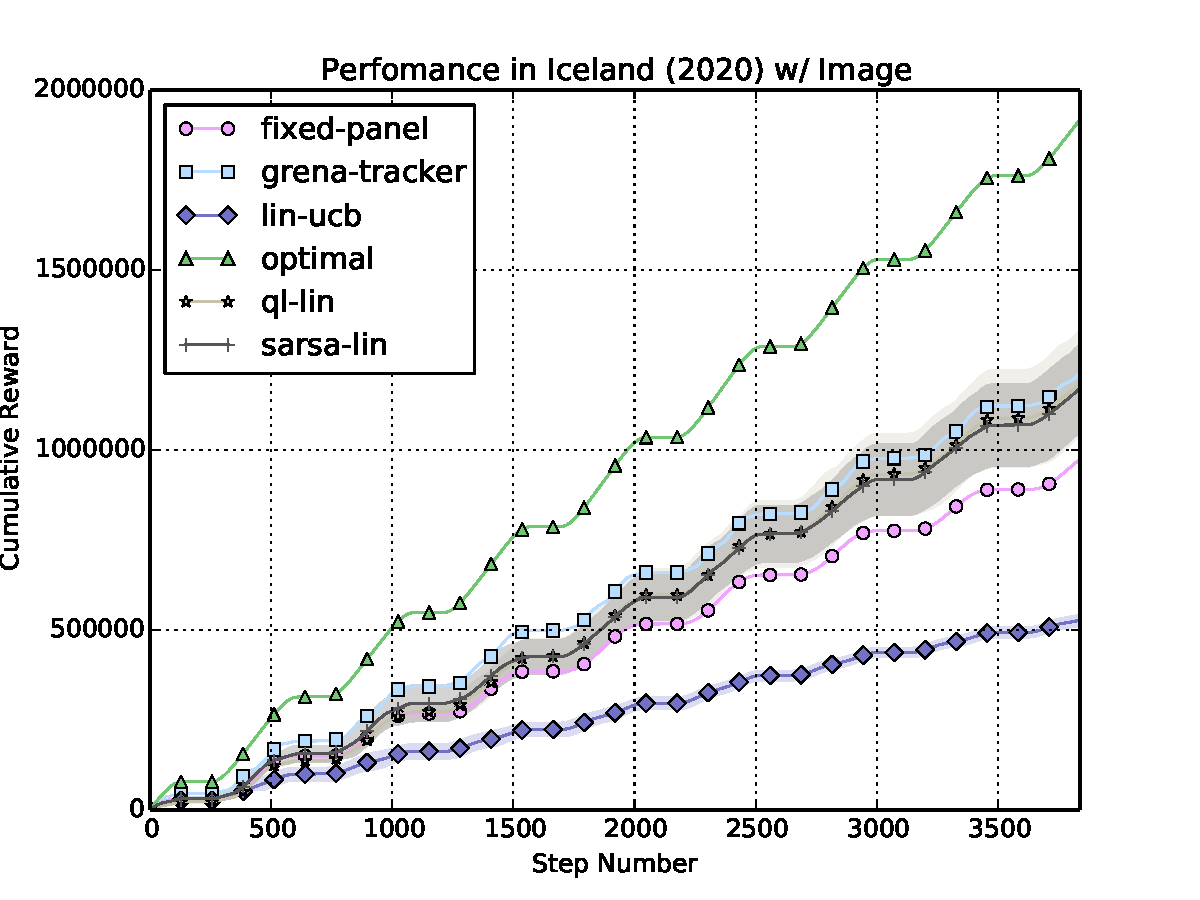
\includegraphics[scale=0.26]{figures/reykjavik/true_cumulative}} \hspace{1mm} % True sun angles percept.
	\subfloat[Bitmap of the Sky]{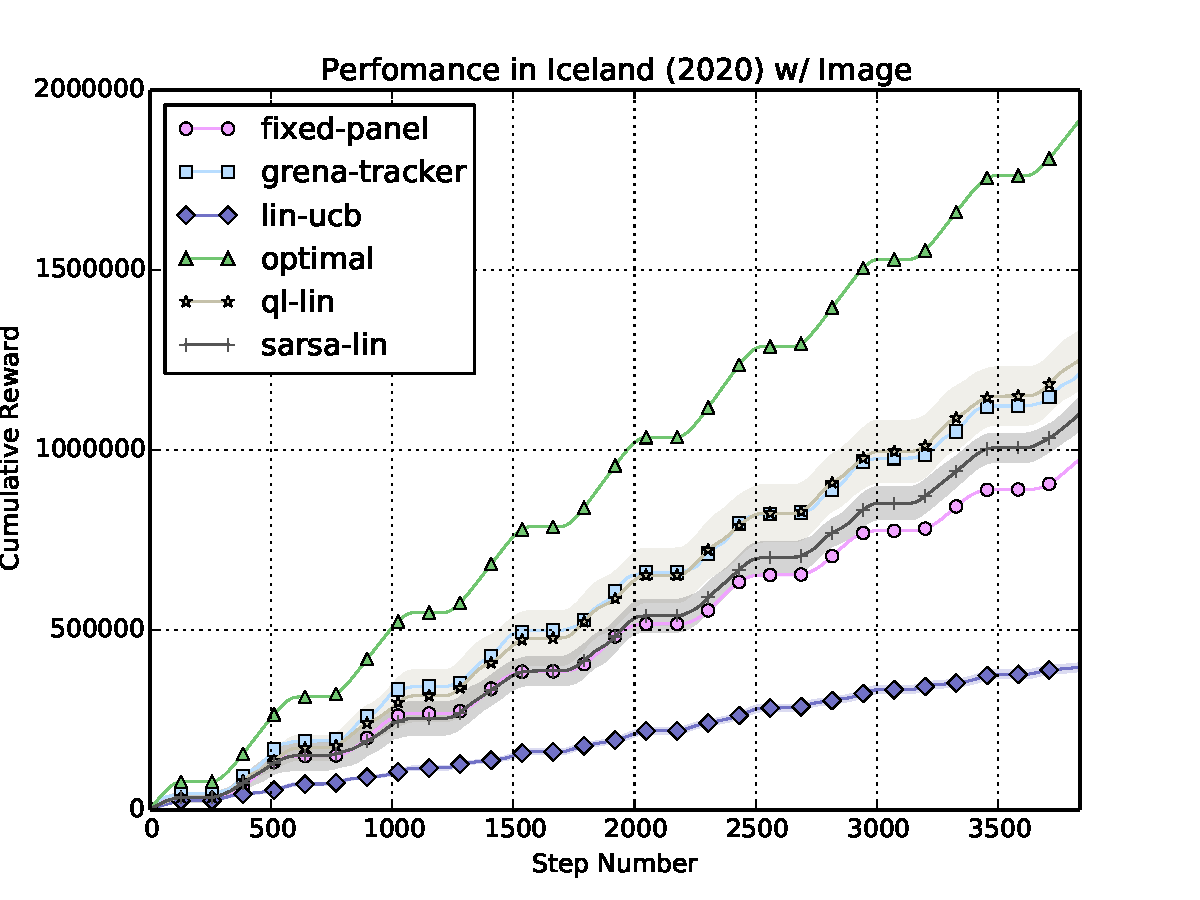
\includegraphics[scale=0.26]{figures/reykjavik/img_cumulative}} \hspace{1mm} % Sun image percept.
	\subfloat[Bitmap of the Cloudy Sky]{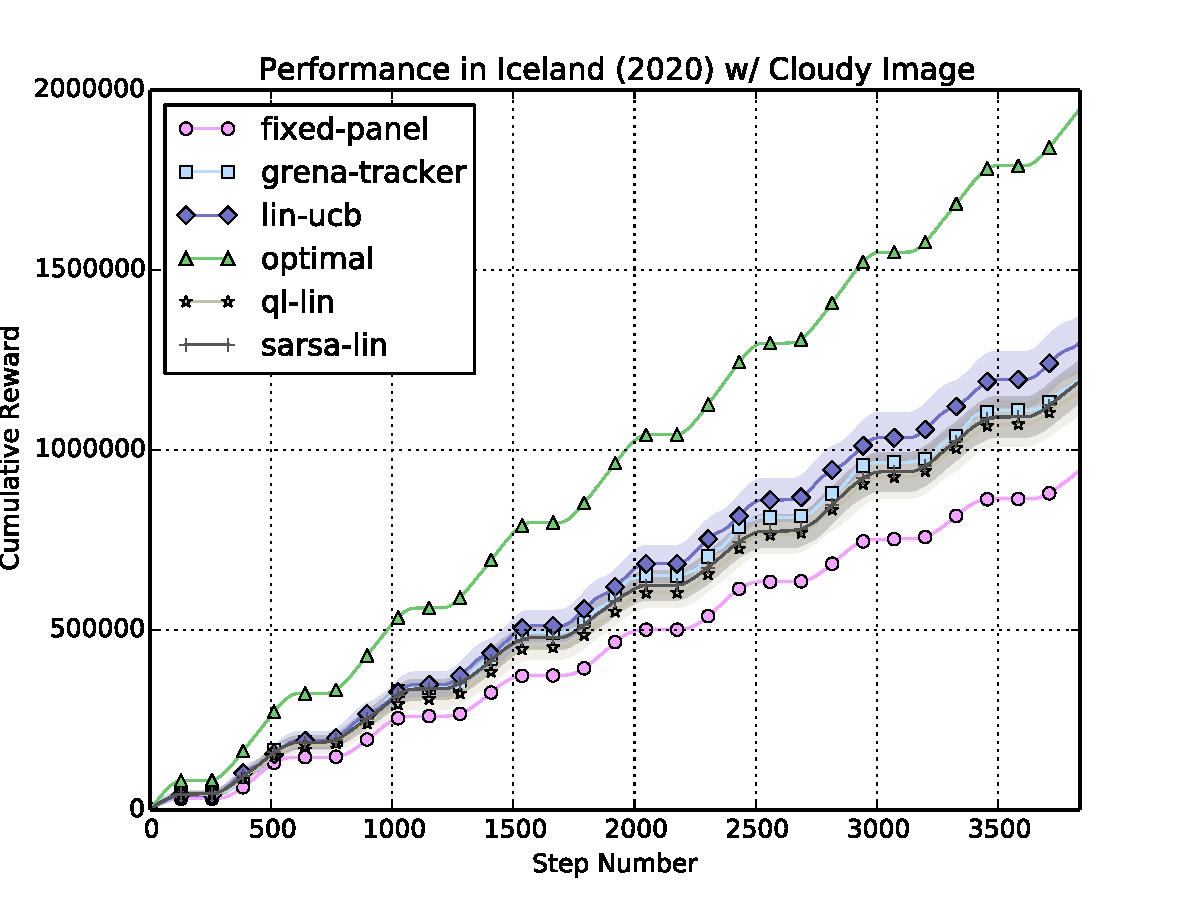
\includegraphics[scale=0.26]{figures/reykjavik/cloud_cumulative}} \\ % Sun image w/ clouds percept.
%	\subfloat[True Sun Angles]{\includegraphics[scale=0.26]{figures/reykjavik/true_avg}} \hspace{1mm} % True sun angles percept.
%	\subfloat[Bitmap of the Sky]{\includegraphics[scale=0.26]{figures/reykjavik/img_avg}} \hspace{1mm} % Sun image percept.
%	\subfloat[Bitmap of the Cloudy Sky]{\includegraphics[scale=0.26]{figures/reykjavik/cloud_avg}} % Sun image w/ clouds percept.
\caption{Cumulative irradiance falling on the panel's surface given different percepts over six days of learning in Reykjavik, Iceland in March of 2018.}
\label{fig:results_ice}
\end{center}
\end{figure*}




% Results (single axis vs dual axis)
\begin{figure}
\begin{center}
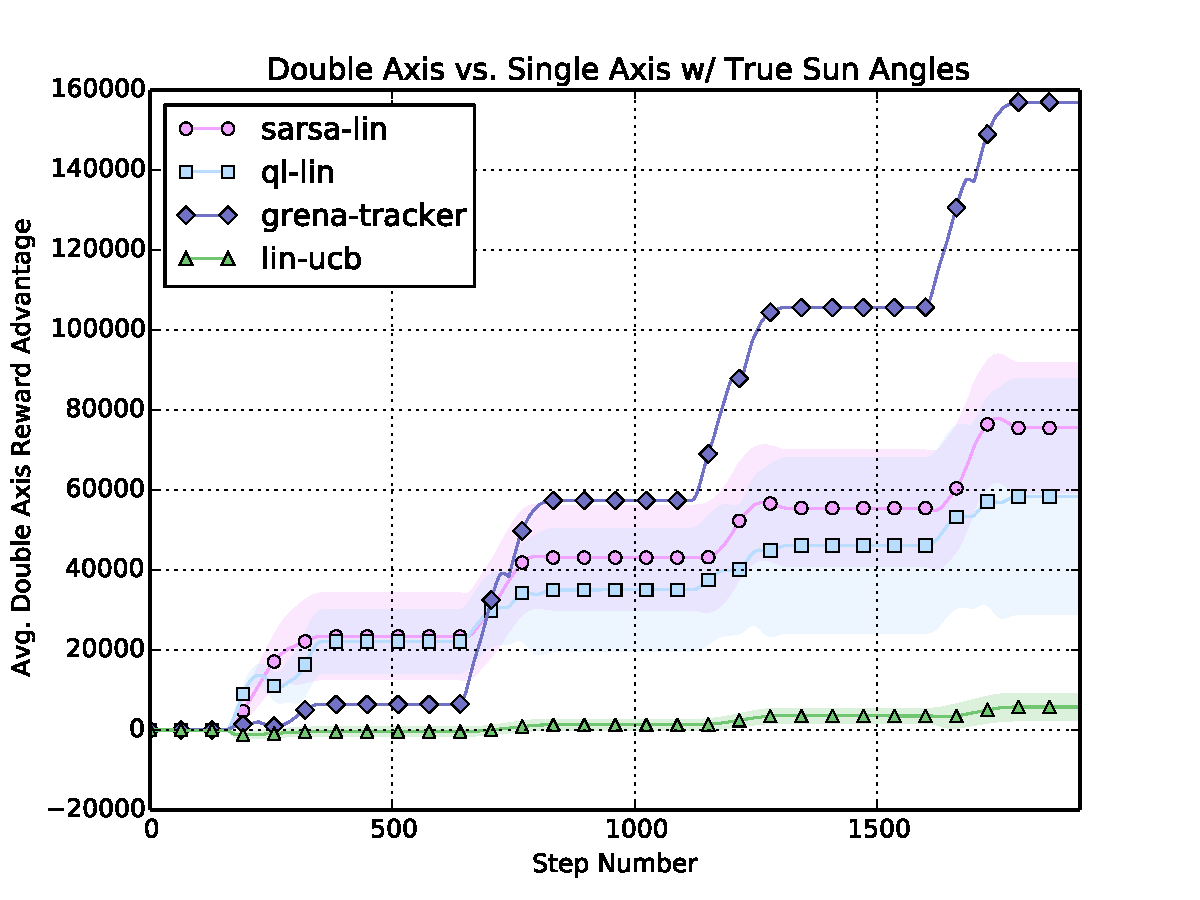
\includegraphics[scale=0.26]{figures/saxis_vs_daxis_true}
\caption{Comparison of single axis to dual axis approach with the true sun percepts.}
\label{fig:results_axis}
\end{center}
\end{figure}


% Results (rho tests)
%\begin{figure*}
%\begin{center}
%\includegraphics[scale=0.26]{figures/saxis_vs_daxis}
%\caption{Effect of ground reflective index on energy acquired.}
%\label{fig:results_rho}
%\end{center}
%\end{figure*}




% -----------------------
% --- Conclusion ---
% -----------------------
\section{Conclusion}

We have here demonstrated the benefits of using the approach of Reinforcement Learning to improve the performance of solar panels. We develop a high fidelity test bed for the problem of solar energy harvesting, capable of simulating solar irradiance models anywhere on Earth with a variety of generated image percepts to approximate real world conditions. We take the simulation, and the evaluation of simple RL approaches on solar panel control to each be of independent interest to the broader AI and computational sustainability communities.

In the future, the clear next step is to implement a functioning RL controller on real solar panels. Additionally, there are several novel algorithmic challenges posed by the solar panel setting. First, both movement and observation expend energy; incorporating these expenditures explicitly into the model poses both challenging planning and exploration questions. Similarly,~\citet{Hsu2015} demonstrate that simple RL approaches can optimize the problem of Maximum Power Point Tracking (MPTT) for solar panels; a system that jointly optimizes over these two criteria poses another difficult challenge. We are also interested in investigating transfer learning between our simulation and the real world, similar to the setup of~\cite{Taylor2007}. 





% ------------------------
% --- Bilbiography ---
% ------------------------
\bibliographystyle{ijcai/named}
\bibliography{../solar}

\end{document}